\documentclass[12pt, a4paper]{article}
\usepackage{caption}
\usepackage{graphicx}
\usepackage{listings}
\usepackage{siunitx}
\usepackage{hyperref}
\def\checkmark{\tikz\fill[scale=0.4](0,.35) -- (.25,0) -- (1,.7) -- (.25,.15) -- cycle;}
\usepackage{tikz-network}
\hypersetup{
    colorlinks,
    citecolor=black,
    filecolor=black,
    linkcolor=black,
    urlcolor=black
}
\usepackage{amsmath, amsfonts, amssymb, amsthm}
\renewcommand{\thesubsubsection}{\thesubsection.\alph{subsubsection}}
\title{Algorithms and datastructures\\Exercises}
\date{2022}
\author{Kristoffer Klokker}
\begin{document}
	\maketitle
	\clearpage
	\tableofcontents
	\clearpage
		\setcounter{section}{5}
		\section{Week}
			\subsection{Indicate the following according to figure 1.}
				\begin{figure}[h!]
					\centering
					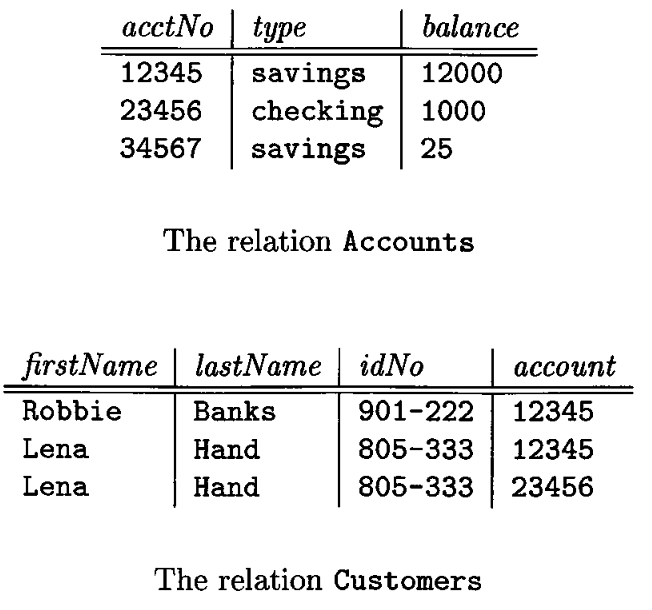
\includegraphics[width=300px]{assets/W6E1.png}
					\caption{Two relations of a banking database}
				\end{figure}
				\subsubsection{The attributes of each realtion}
					Accounts: $acctNo$, $type$, $balance$\\
					Customers: $firstName$, $lastName$, $idNo$, $account$
				\subsubsection{The tuples of each realtion}
					\begin{itemize}
						\item $12345, savings, 12000$
						\item $23456, checking, 1000$
						\item $34567, savings, 25$\\[5mm]
						\item $Robbie$, $Banks$, $901-222$, $12345$
						\item $Lena$, $Hand$, $805-333$, $12345$
						\item $Lena$, $Hand$, $805-333$, $23456$ 
					\end{itemize}
				\subsubsection{The components of one tuble of each realtion}
					$12000$\\
					$Banks$
				\subsubsection{The relation schema of each realtion}
					$Accounts(acctNo, type, balance)$\\
					$Customers(firstName, lastName, idNo,account)$
				\subsubsection{The database schema}
					$Accounts, Customers$
				\subsubsection{A suitable domain of each attribute}
					\begin{itemize}
						\item $acctNo$ - $INT$
						\item $type$ - $VARCHAR[20]$
						\item $balance$ - $INT$
						\item $firstName$ - $VARCHAR[20]$
						\item $lastName$ - $VARCHAR[20]$
						\item $idNo$ - $CHAR[7]$
						\item $account$ - $INT$
					\end{itemize}
				\subsubsection{Another equivalent way to present each relation.}
					The attributes could simply just be in a different order.
			\subsection{In a table with the following attributes which are valid example of keys}
				$$title, year, length, genre, studioName, producerC\#$$
				\begin{itemize}
					\item title, year
					\item title, year, studioName
					\item title, length
					\item length, genre, studioName, year
				\end{itemize}
			\subsection{How many ways can relation be represented if it has:}
				\subsubsection{Four attributes and five tuples}
					$4! \cdot 5! = 2880$\\
				\subsubsection{$n$ attributes and $m$ tuples}
					$n! \cdot m!$
			\subsection{Write a database schema of the following relations}
				The datasbase schema includes\\
				$Product(make, model, type)$\\
				$PC(model, speed,ram hd, price)$\\
				$Laptop(model, speed, ram, hd ,screen, price)$\\
				$Printer(model, color, type, price)$
				\subsubsection{Write a schema for $Product$}
					CREATE TABLE Product(VARCHAR[20] maker, INT model, INT type)\\
					The type is here an int where 0 is PC, 1 is laptop and 2 is printer. There is no foreign keys due to it being the lookup table for the other relations
				\subsubsection{Write a schema for $PC$}
					CREATE TABLE PC(INT model, FLOAT speed, INT ram, BOOLEAN hd, FLOAT prize, FOREIGN KEY(Products) REFERENCES Products(model))\\
					Here the model is a reference to products, speed is gigahertz of CPU
				\subsubsection{Write a schema for $Printer$}
					CREATE TABLE Printer(INT model, BOOLEAN color, VARCHAR[20] type, FLOAT price, FOREIGN KEY(Products) REFERENCES Products(model))\\
				\subsubsection{Write an alternation for Printer and delete the attribute color}
					ALTER TABKE Printer DROP color 
				\subsubsection{Add an $od$ attribute for PC, which defaults to none an otherwise can be cd or dvd}
					ALTER TABLE PC ADD VARCHAR[20] od DEFAULT 'none'
		\section{Week}
			\subsection{Working with linear notation}
				The following exercises uses the following schema:\\
				$Product(maker, model, type)$\\
				$PC(model, speed,ram, hd, price)$\\
				$Laptop(model, speed, ram, hd ,screen, price)$\\
				$Printer(model, color, type, price)$
				\subsubsection{PC models which have speed of at least 3.00?}
					$\pi_{model}(\sigma_{speed > 3.00}(PC))$
				\subsubsection{PC manufacturers which makes PC with a hdd with at leat 100GB}
					$\pi_{maker}(Product \bowtie \sigma_{hd >= 100}(PC))$
				\subsubsection{Find model and price of all products made by manufacturer $B$}
					\begin{align*}
						man &:= \sigma_{maker = B}(Product)\\
						PCModelPrice &:= \pi_{model, price}(man \bowtie PC)\\
						LaptopModelPrice &:= \pi_{model, price}(man \bowtie Laptop)\\
						PrinterModelPrice &:= \pi_{model, price}(man \bowtie Printer)\\
						modPrice &:= PCModelPrice \cup LaptopModelPrice \cup PrinterModelPrice
					\end{align*}
				\subsubsection{Find model numbers of all color laster printers}
					$\pi_{model}(\sigma_{color = 1 AND type = laser}(Printer))$
				\subsubsection{Find manufactures that sell Laptops but not PC}
					Due to algebra not including a method for group by I have answered in form of SQL queries.\\
					SELECT (SELECT maker FROM LAPTOP NATURAL JOIN Product GROUP BY maker)  -  (SELECT maker FROM PC NATURAL JOIN Product GROUP BY maker)
				\subsubsection{Find hd size which accour in two or more PC's}
					\begin{align*}
						PC = \pi_{model,hd}(PC)\\
						PC2(model2,hd) = \pi_{model,hd}(PC)\\
						hd = \pi_{hd}(\sigma_{model != model2}(PC \bowtie PC2)
					\end{align*}
				\subsubsection{Find PC models which have the same speed and RAM, a pair should only be listed once}
					\begin{align*}
						Model1 = \pi_{model,speed,RAM}(PC)\\
						Model2(model2,speed,RAM) = \pi_{model,speed,RAM}(PC)\\
						models = \pi_{model,model2}(\sigma_{model != model2}(PC \bowtie PC2)
 					\end{align*}			
				\subsubsection{Find PC models which have the same speed and RAM, a pair should only be listed once}
					\begin{align*}
						ModelPC = \pi_{model}\sigma_{speed >= 2.8}(PC)\\
						ModelLaptop = \pi_{model}\sigma_{speed >= 2.8}(Laptop)\\
						models = ModelPC \cup ModelLaptop\\
						mans = \pi_{maker,model}(models \bowtie Product)\\
						twoProduct = \sigma_{maker2 = maker and model2 != model}(\rho_{maker2,model2}mans \times mans)
 					\end{align*}			
				\subsubsection{Find manufactore(s) of the fastest PC or laptop}
					\begin{align*}
						computers = \pi_{model,speed}Laptop \cup PC\\
						computers2(model2, speed2) = computers\\
						slowSpeed = \pi_{speed}(computers\bowtie_{speed<speed2} computers2)\\
						fastSpeed(fast) = \pi_{speed}(computers)-slowSpeed\\
						fastModels = computers \bowtie_{speed=fast} fastSpeed\\
						mans = \pi_{maker}(fastModels \bowtie Product)
 					\end{align*}	
				\subsubsection{Find manufactores who sellf at lest three PC's}
					\begin{align*}
						model = \rho_{model}PC\\
						computers = model \times model(model2) \times model(model3)\\
						models = \sigma_{model = model2 and model2 = model3}(computers)\\
						mans = \pi_{maker}(models \bowtie Product)
 					\end{align*}		
				\subsubsection{Find manufactores who sell atleast 3 different speed PC's}
					\begin{align*}
						model = \rho_{model}PC\\
						computers = model \times model(model2) \times model(model3)\\
						models = \sigma_{model = model2 and model2 = model3}(computers)\\
						mans = \pi_{maker}((models \bowtie Product)
 					\end{align*}	
				\subsubsection{Find manufactores who sell exactly three PC's}
					\begin{align*}
						model = \rho_{model}PC\\
						computers = model \times model(model2) \times model(model3)\\
						models = \sigma_{model = model2 and model2 = model3}(computers)\\
						TooManycomputers = model \times model(model2) \times model(model3) \times model(model4)\\
						models = \sigma_{model = model2 and model2 = model3}(computers)\\
						TooManymodels = \sigma_{model = model2 and model2 = model3 and model3 = model4}(computers)\\
						mans = \pi_{maker}((models \bowtie Product)
 					\end{align*}											
			\clearpage
			\subsection{In the following data, what is the result of $\pi_{speed}(PC)$ when treated as a bag and set}
				\begin{table}[h!]
				\begin{tabular}{|l|l|l|l|l|}
				\hline
				model & speed &ram &hd &price  \\\hline
				1001 &2.66 &1024 &250 &2114 \\\hline
				1002 &2.10 & 512 &250 &995   \\\hline
				1003 &1.42 & 512 & 80 &478      \\\hline
				1004 &2.80 &1024 &250 &649    \\\hline
				1005 &3.20 &512 &250 &630     \\\hline
				1006 &3.20 &1024 &320 &1049   \\\hline
				1007 &2.20 & 1024 &200 &510  \\\hline
				1008 &2.20 &2048 &250 &770  \\\hline
				1009 &2.00 &1024 &250 &650  \\\hline
				1010 &2.80 &2048 &300 &770    \\\hline
				1011 &1.86 &2048 &160 &959  \\\hline
				1012 &2.80 &1024 &160 &649    \\\hline
				1013 &3.06 &512 &80 &529     \\\hline
				\end{tabular}
				\end{table}
				\begin{minipage}[t]{0.5\textwidth}
				\begin{center}
				Bag\\
				\begin{tabular}{|l|}
				\hline
				speed\\\hline
				2.66 \\\hline
				2.10 \\\hline
				1.42 \\\hline
				2.80 \\\hline
				3.20 \\\hline
				3.20 \\\hline
				2.20 \\\hline
				2.20 \\\hline
				2.00 \\\hline
				2.80 \\\hline
				1.86 \\\hline
				2.80 \\\hline
				3.06 \\\hline
				\end{tabular}
				\end{center}
				\end{minipage}
				\begin{minipage}[t]{0.5\textwidth}
				\begin{center}
				Set\\
				\begin{tabular}{|l|}
				\hline
				speed\\\hline
				2.66 \\\hline
				2.10 \\\hline
				1.42 \\\hline
				2.80 \\\hline
				3.20 \\\hline
				2.20 \\\hline
				2.00 \\\hline
				2.80 \\\hline
				1.86 \\\hline
				3.06 \\\hline
				\end{tabular}
				\end{center}
				\end{minipage}
	\section{Week}
		\subsection{In the query SELECT A B is b an attribute or alias}
			B will be an alias for it to be an attribute A and B has to be comma seperated.
		\subsection{Write the following queries based on the following tables}
			Movies(title , year, length, genre, studioName, producerC$\#$)\\
			StarsIn(movie Title , movieYear, starName)\\
			MovieStar(name, address, gender, birthdate )\\
			MovieExec(name, address, cert$\#$ , netWorth)\\
			Studio(name, address , presC$\#$)
			\subsubsection{Find the address of MGM studios}
				SELECT address FROM Studio WHERE name = 'MGM'
			\subsubsection{Find Sandra Bullock's birthday}
				SELECT birthdate FROM MovieStar WHERE name = 'Sandra Bullock'
			\subsubsection{Find all the stars that appeared either in a movie made in 1980 or a movie with Love in the title}
				SELECT Star.name FROM MovieStar Star WHERE Star.name IN (SELECT starName FROM StarsIn, Movies WHERE MovieTitle = title AND (Movies.title LIKE $\%$Love$\%$' OR Movies.year = 1980))
			\subsubsection{Find all executive worth at least \$10,000,000}
				SELECT name FROM MovieExec WHERE netWorth $>$ 10000000
			\subsubsection{Find all the stars who either are male or live in Malibu}
				SELECT name FROM MovieStar WHERE gender = 'male' OR address LIKE '$\%$Malibu$\%$'  
			\subsubsection{Who were the male stars in $Titanic$}
				SELECT name FROM Movies, StarsIn, MovieStar WHERE title = 'Titanic' AND title = movieTitle AND starName = name AND gender = male
			\subsubsection{Which stars appeared in movies produced by MGM in 1995}
				SELECT starName FROM Movies, StarsIn WHERE studioName = 'MGM' AND title = movieTitle
			\subsubsection{Who is the presiden of MGM Studios}
				SELECT MovieExec.name FROM Studio, MovieExec WHERE Studio.name = 'MGM' AND presC$\#$ = cert$\#$
			\subsubsection{Which movies are longer than $Gone with the Wind$}
				SELECT title FROM Movies WHERE length $>$ (SELECT length FROM MOVIES WHERE title = 'Gone with the Wind')
			\subsubsection{Which executive are worth more than Merv Griffin}
				SELECT name FROM MovieExec WHERE netWorth $>$ (SELECT netWorth FROM MovieExec WHERE name = 'Merv Griffin')
		\subsection{Describe possible values for a and b in the following conditions to be true}
			\subsubsection{a = 10 OR b = 20}
				a is 10, b can be anything including null, and the otherway around
			\subsubsection{a = 10 AND b = 20}
				Both a has to be 10 and b has to be 20
			\subsubsection{a $<$ 10 OR a $>$= 10}
				One of the statements has to be true where the other can both be UNKNOWN by being null or just FALSE be being 11 or higher ot just TRUE.
			\subsubsection{a = b}
				This will only be true if both have the same value, in case of null it will return UNKNOWN
			\subsubsection{a $<=$ b}
				If b is higher than a or equal to a it will return true. If one them is null it will be UNKNOWN an otherwise it will be false.
		\subsection{Write the following queries based on the following tables}
			Product(maker, model, type)\\
			PC(model, speed, ram, hd, price)\\
			Laptop(model, speed, ram, hd, screen, price)\\
			Printer(model, color, type, price)\\
			\subsubsection{Find the makers of PC's with a speed of at least 3.0}
				SELECT model FROM PC WHERE speed $>$ 3.0
			\subsubsection{Find the printers with the highest price}
				SELECT model FROM Printer WHERE price = (SELECT MAX(price) FROM Printer)
			\subsubsection{Find the laptops whose speed is slower than that of any PC}
				SELECT model FROM Laptop WHERE speed < (SELECT MIN(speed) FROM PC)
			\subsubsection{Find the model number of the item (PC, Laptop, Printer) with the highest price}
				SELECT model FROM \\
					(SELECT model, price FROM PC UNION SELECT model,price FROM Laptop UNION SELECT model,price FROM Printer) \\
					WHERE price = SELECT MAX(price) FROM \\
						(SELECT MAX(price) FROM PC) UNION (SELECT MAX(price) FROM Laptop) UNION  (SELECT MAX(price) FROM Printer)) 
			\subsubsection{Find the maker of the color printer with lowest price}
				SELECT model FROM Printer WHERE type=color AND price = (SELECT MIN(price) FROM Printer)
	\section{Week}
		\subsection{Write SQL queries for the following database}
			$Product(maker, model, type)$\\
			$PC(model, speed,ram, hd, price)$\\
			$Laptop(model, speed, ram, hd ,screen, price)$\\
			$Printer(model, color, type, price)$
			\subsubsection{What PC models have a speed grater than 3}
				SELECT * FROM PC WHERE speed $>$ 3
			\subsubsection{Find model and price for all products made by manufacturer B}
				SELECT price, model FROM PC, Laptop, Printer Where model EXISTS (SELECT model FROM product WHERE maker = B)
			\subsubsection{Find manufactureres of at least two different computers with speed grather than 2.8}
				SELECT maker FROM (SELECT maker FROM Product WHERE model EXIST (SELECT models FROM PC, Laptop Where speed $>$ 2.8)) WHERE COUNT(maker) $>$= 2		
			\subsubsection{Find the average speed of PC's}
				SELECT AVG(speed) FROM PC
			\subsubsection{Find the average speed of laptops costing over \$1000}
				SELECT * FROM Laptops WHERE price $>$ 1000
			\subsubsection{Find the average price of PC's and Laptops made by manufacturer "D"}
				SELECT AVG(price) FROM Laptop, PC WHERE model EXIST (SELECT model FROM Product WHERE maker = 'D')
			\subsubsection{Find for each different speed, the average price of a PC}
				SELECT AVG(price) FROM PC GROUP BY speed
			\subsubsection{Find for each manufacturer the average screen size of its laptops}
				SELECT AVG(screen) FROM PC NATURAL JOING Product GROUP BY maker
			\subsubsection{Find the manufacturers that make at least three different model of PC}
				SELECT maker FROM PC NATURAL JOIN Product GROUP BY maker HAVING COUNT(*) $>$ 2
			\subsubsection{Find for each manufacturer who selss PC's the maximum price of a PC.}
				SELECT MAX(price) FROM PC NATURAL JOIN Product GROUP BY maker
			\subsubsection{Find for each speed of PC above 2.0 the average price}
				SELECT AVG(price) FROM PC GROUP BY speed HAVING speed $>$ 2
			
				
				
					
				
			
\end{document}


